\chapter{Conclusiones Generales} 

En la presente tesis se realizaron aportes en la investigación de materiales nanoestructurados y sus posibles aplicaciones en el marco de las energías limpias y renovables. Como la principal fuente de energía que llega a la Tierra es el sol, constituyendo así un recurso inmenso e inacabable, es fundamental el estudio de la interacción de la luz con la materia para entender cuál es la mejor manera en la que puede ser aprovechada.  

Nanoestructuras semiconductoras como NP de TiO$_2$ o nw de ZnO fueron estudiadas a lo largo de este trabajo, las cuales fueron sensibilizadas con colorantes para captar la energía del sol. Esto último es importante de resaltar ya que los SC mencionados son transparentes a la luz visible pero con la absorción de moléculas en su superficie se produce un cambio en la estructura electrónica de ambos, lo cual se ve reflejado en la estructura de bandas o propiedades ópticas como se analizó detalladamente en el capítulo 5.

Las DSSC son, a grandes rasgos, nanoestructuras sensibilizadas inmersas en una celda electroquímica. Diversos parámetros se tienen en cuenta a la hora de confeccionar una DSSC y por eso la selección estratégica de los materiales es fundamental. La eficiencia general de conversión de luz solar a energía eléctrica de una DSSC se puede expresar como el producto de tres términos clave \cite{Kalyanasundaram}: 

\begin{equation}
 H = \eta_{abs}. \eta_{inj}.\eta_{coll}
\end{equation}

donde $\eta_{abs}$ es la eficiencia de absorción de luz por el colorante, $\eta_{inj}$ es la eficiencia de la inyección de carga desde el estado excitado del colorante, y $\eta_{coll}$ es la eficiencia de recolección de carga en la capa de óxido mesoporoso. En el marco de las simulaciones computacionales utilizadas en esta tesis, calculamos espectros de absorción óptica y transferencia de carga, lo cual brinda contribuciones al cálculo de $\eta_{abs}$ y $\eta_{inj}$, mientras que no hemos profundizado en la eficiencia $\eta_{coll}$ con estos métodos.

Un fotosensibilizador ideal será el que absorba toda la luz solar en la región del visible-IR cercano con un alto coeficiente de absorción. A lo largo del trabajo se analizaron 3 colorantes: ALZ, FSD101 y CAT, de los cuales sólo los dos primeros absorben en el visible mientras que el tercero absorbe en el UV cuando están aislados. Esto indica a priori que ALZ y FSD101 recolectan más eficientemente la luz solar. Sin embargo, se ha demostrado en esta tesis como en trabajos anteriores que la adsorción del colorante CAT a la superficie de los SC utilizados produce la aparición de una nueva banda en la zona del visible del espectro, lo cual no ocurre con las demás moléculas. A la hora de elegir un colorante también son deseables otras propiedades que han sido nombradas a lo largo de la tesis como es la disposición energética adecuada de los orbitales HOMO-LUMO de la molécula que permita la inyección cuantitativa de cargas del colorante al SC o viceversa. Las energías de estos orbitales y su comparación con las bandas del SC se pueden obtener mediante simulaciones computacionales y en consecuencia orientarnos con respecto a la selección del colorante. 

Para una transferencia de electrones eficiente se requiere un buen acoplamiento electrónico entre el SC y el fotosensibilizador. En este caso, se demostró que el CAT tiene un mayor acoplamiento con la NP de TiO$_2$ (capítulo 4) y con el nw de ZnO (capítulo 5) y por ende mayor transferencia de carga en ambos casos con respecto a otros colorantes analizados. En el capítulo 4 se calculó la eficiencia de la transferencia de carga en sistemas CAT-NP obteniendo un valor que supera ampliamente las eficiencias de los otros complejos y este resultado está directamente relacionado con el mecanismo por el cuál se lleva a cabo la transferencia de carga. Sin embargo, a pesar de las ventajas que presenta el colorante, las eficiencias globales de las DSSC basadas en CAT son bajas. Muchos trabajos \cite{Ooyama2017,Wang2003,Ramakrishna2001,Huber2000} afirman que este resultado se debe a la rápida recombinación de carga de los electrones inyectados en el electrodo semiconductor al colorante oxidado.  

Como mencionamos a lo largo de la tesis, las DSSC pueden ser de tipo-n o tipo-p, es decir compuestas por semiconductores tipo-n o tipo-p, respectivamente. Por otro lado la transferencia de carga que ocurre entre el colorante y el SC puede llevarse a cabo de forma directa o indirecta dependiendo del grado de acoplamiento entre las dos partes. El modelo que se presentó en el capítulo 1, puede representar cualquier sistema colorante adsorbido a un semiconductor no periódico como por ejemplo sistemas colorante-NP. En la figura \ref{comp} a la derecha se muestran los espectros de absorción del CAT aislado y del complejo CAT-NP de TiO$_2$ simulados con dftb+. Este sistema cuenta con un colorante con energía de excitación H-L mayor al GAP del SC. En la figura \ref{comp} a la derecha se muestran los espectros de absorción de una molécula diatómica aislada y de un complejo diatómica-SC no periódico. Los parámetros del modelo TB se ajustaron de forma que representen el sistema CAT-NP, es decir con un gran acoplamiento entre la molécula diatómica y el SC o, en otras palabras, $\gamma = 0.1$ y un valor de $\delta$ lo suficientemente grande como para que la energía H-L sea mayor al GAP. Al comparar los espectros obtenidos mediante los dos métodos, observamos en ambos casos la aparición de una nueva banda a bajas energías y que la banda del colorante no se aprecia debido a que absorbe en la misma zona que el SC. 

\begin{figure}[!htb]
\centering
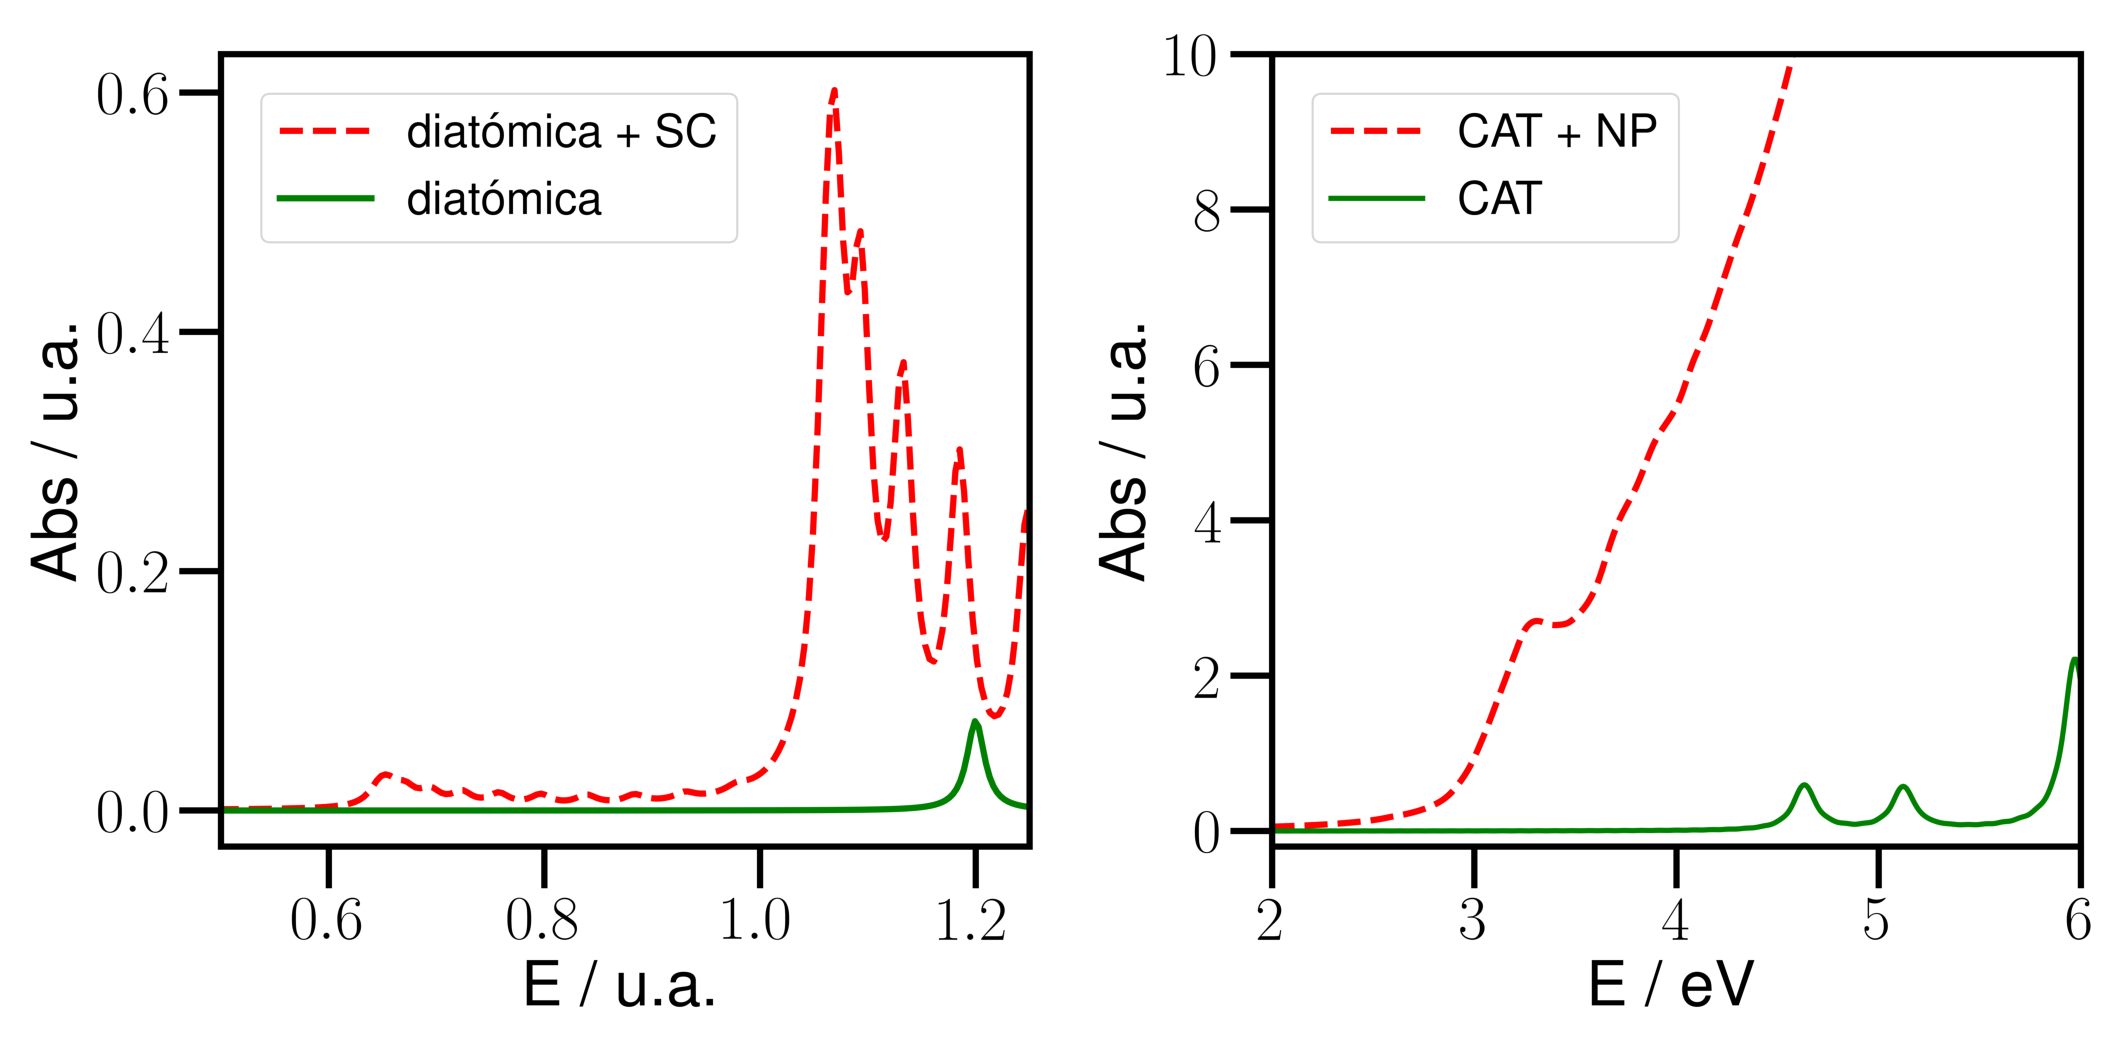
\includegraphics[height=6cm]{cap7/figs/comp_modelo_directo.eps}
\caption{(\textbf{Izquierda}) espectros de absorción para una diatómica y el complejo diatómica-SC simulados mediante un modelo simple TB y (\textbf{derecha}) espectros de absorción para el CAT y el complejo CAT-NP simulados con dftb+}
\label{comp}
\end{figure}


Los SC utilizados en este trabajo (TiO$_2$ anatasa y ZnO wurtzita) son buenos candidatos para fotoelectrodos en una DSSC ya que ambos son amigables con el medio ambiente, tienen similares GAP y energía de borde de la BC. En comparación al TiO$_2$, el ZnO tiene una mayor movilidad de electrones y menor estabilidad química, ya que se disuelve en condiciones ácidas y básicas \cite{Hagfeldt2010}. La película de NP de TiO$_2$ en las DSSC es un enfoque tradicional, ampliamente utilizado, sin embargo, la relativa facilidad de sintetizar ZnO altamente cristalino con diferentes morfologías (en la estructura wurtzita) ha permitido el uso e investigación de nw de ZnO como fotoánodos. En particular, para investigar los complejos CAT-nw de ZnO en esta tesis fue fundamental contar con un método computacional como el TD-DFTB capaz de calcular propiedades ópticas para sistemas periódicos con un costo computacional relativamente bajo. Al modelar sistemas con condiciones periódicas de contorno podemos elegir una celda pequeña que represente toda la superficie, lo cual permitió en este caso simular sistemas colorante-nw de ZnO con un gran cubrimiento de colorante. Si bien en este trabajo se consideró la adsorción de catecol en forma cis, es decir las moléculas dispuestas unas arriba de otras, a la superficie del nw, no es la única forma a la cuál se une el catecol. Sin embargo, esta configuración más estable según dftb+ mostró una interacción entre orbitales moleculares que en otras configuraciones no se observa.  


Utilizar dinámica molecular como otro método de simulación tuvo el objetivo de incorporar realismo a las simulaciones. Este objetivo se llevó a cabo teniendo en cuenta el efecto de la temperatura y además considerar las interacciones del nw con moléculas de agua debido a las trazas presentes en DSSC a base de electrolitos orgánicos. Es importante considerar estas interacciones para averiguar si las mismas interfieren en la eficiencia global de la celda. 

Los métodos computacionales utilizados en esta tesis no representan todos las variables que se deben tener en cuenta a la hora de calcular valores de eficiencia en las DSSC, sin embargo se pueden estudiar detalladamente los procesos que involucren SC y colorante como son los cálculos de propiedades ópticas y estructura electrónica, los cuales pueden orientar a experimentalistas a la hora de confeccionar una DSSC.
